\section{mo\-Algo$<$ EOT $>$ Class Template Reference}
\label{classmo_algo}\index{moAlgo@{moAlgo}}
Description of an algorithm of the paradiseo-mo library.  


{\tt \#include $<$mo\-Algo.h$>$}

Inheritance diagram for mo\-Algo$<$ EOT $>$::\begin{figure}[H]
\begin{center}
\leavevmode
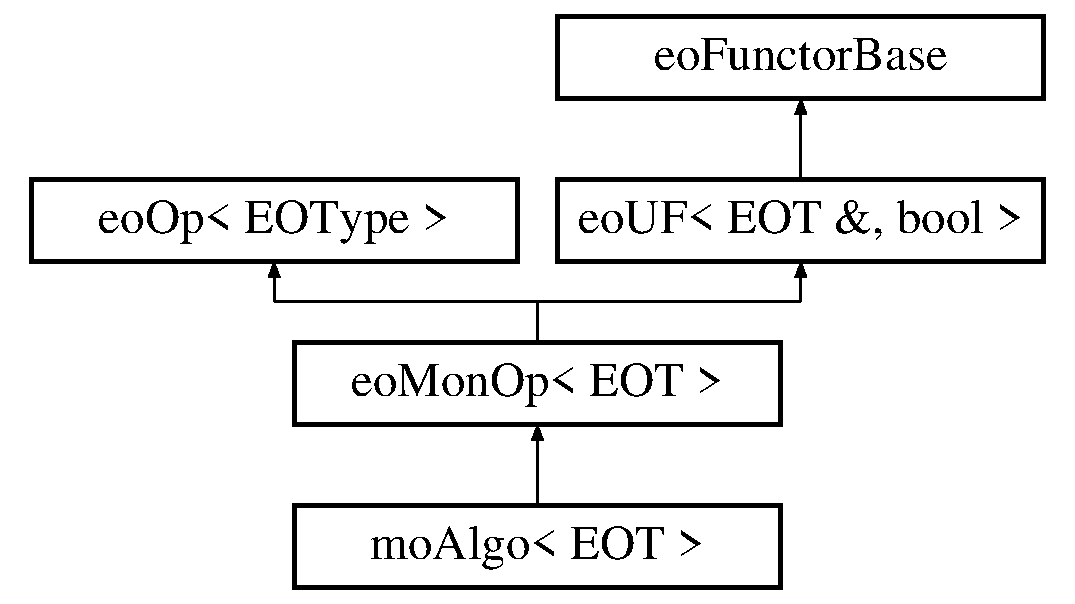
\includegraphics[height=4cm]{classmo_algo}
\end{center}
\end{figure}


\subsection{Detailed Description}
\subsubsection*{template$<$class EOT$>$ class mo\-Algo$<$ EOT $>$}

Description of an algorithm of the paradiseo-mo library. 

{\bf mo\-HC}{\rm (p.\,\pageref{classmo_h_c})}, {\bf mo\-TS}{\rm (p.\,\pageref{classmo_t_s})} and {\bf mo\-SA}{\rm (p.\,\pageref{classmo_s_a})} are 3 examples of algorithm of the paradiseo-mo library. 



Definition at line 46 of file mo\-Algo.h.

The documentation for this class was generated from the following file:\begin{CompactItemize}
\item 
mo\-Algo.h\end{CompactItemize}
